\documentclass{article}
\usepackage[utf8]{inputenc}
\usepackage{graphicx}
\usepackage{titlepic}
\usepackage{hyperref}
\usepackage{xcolor}
\usepackage{amsmath}
\usepackage{textcomp}

\titlepic{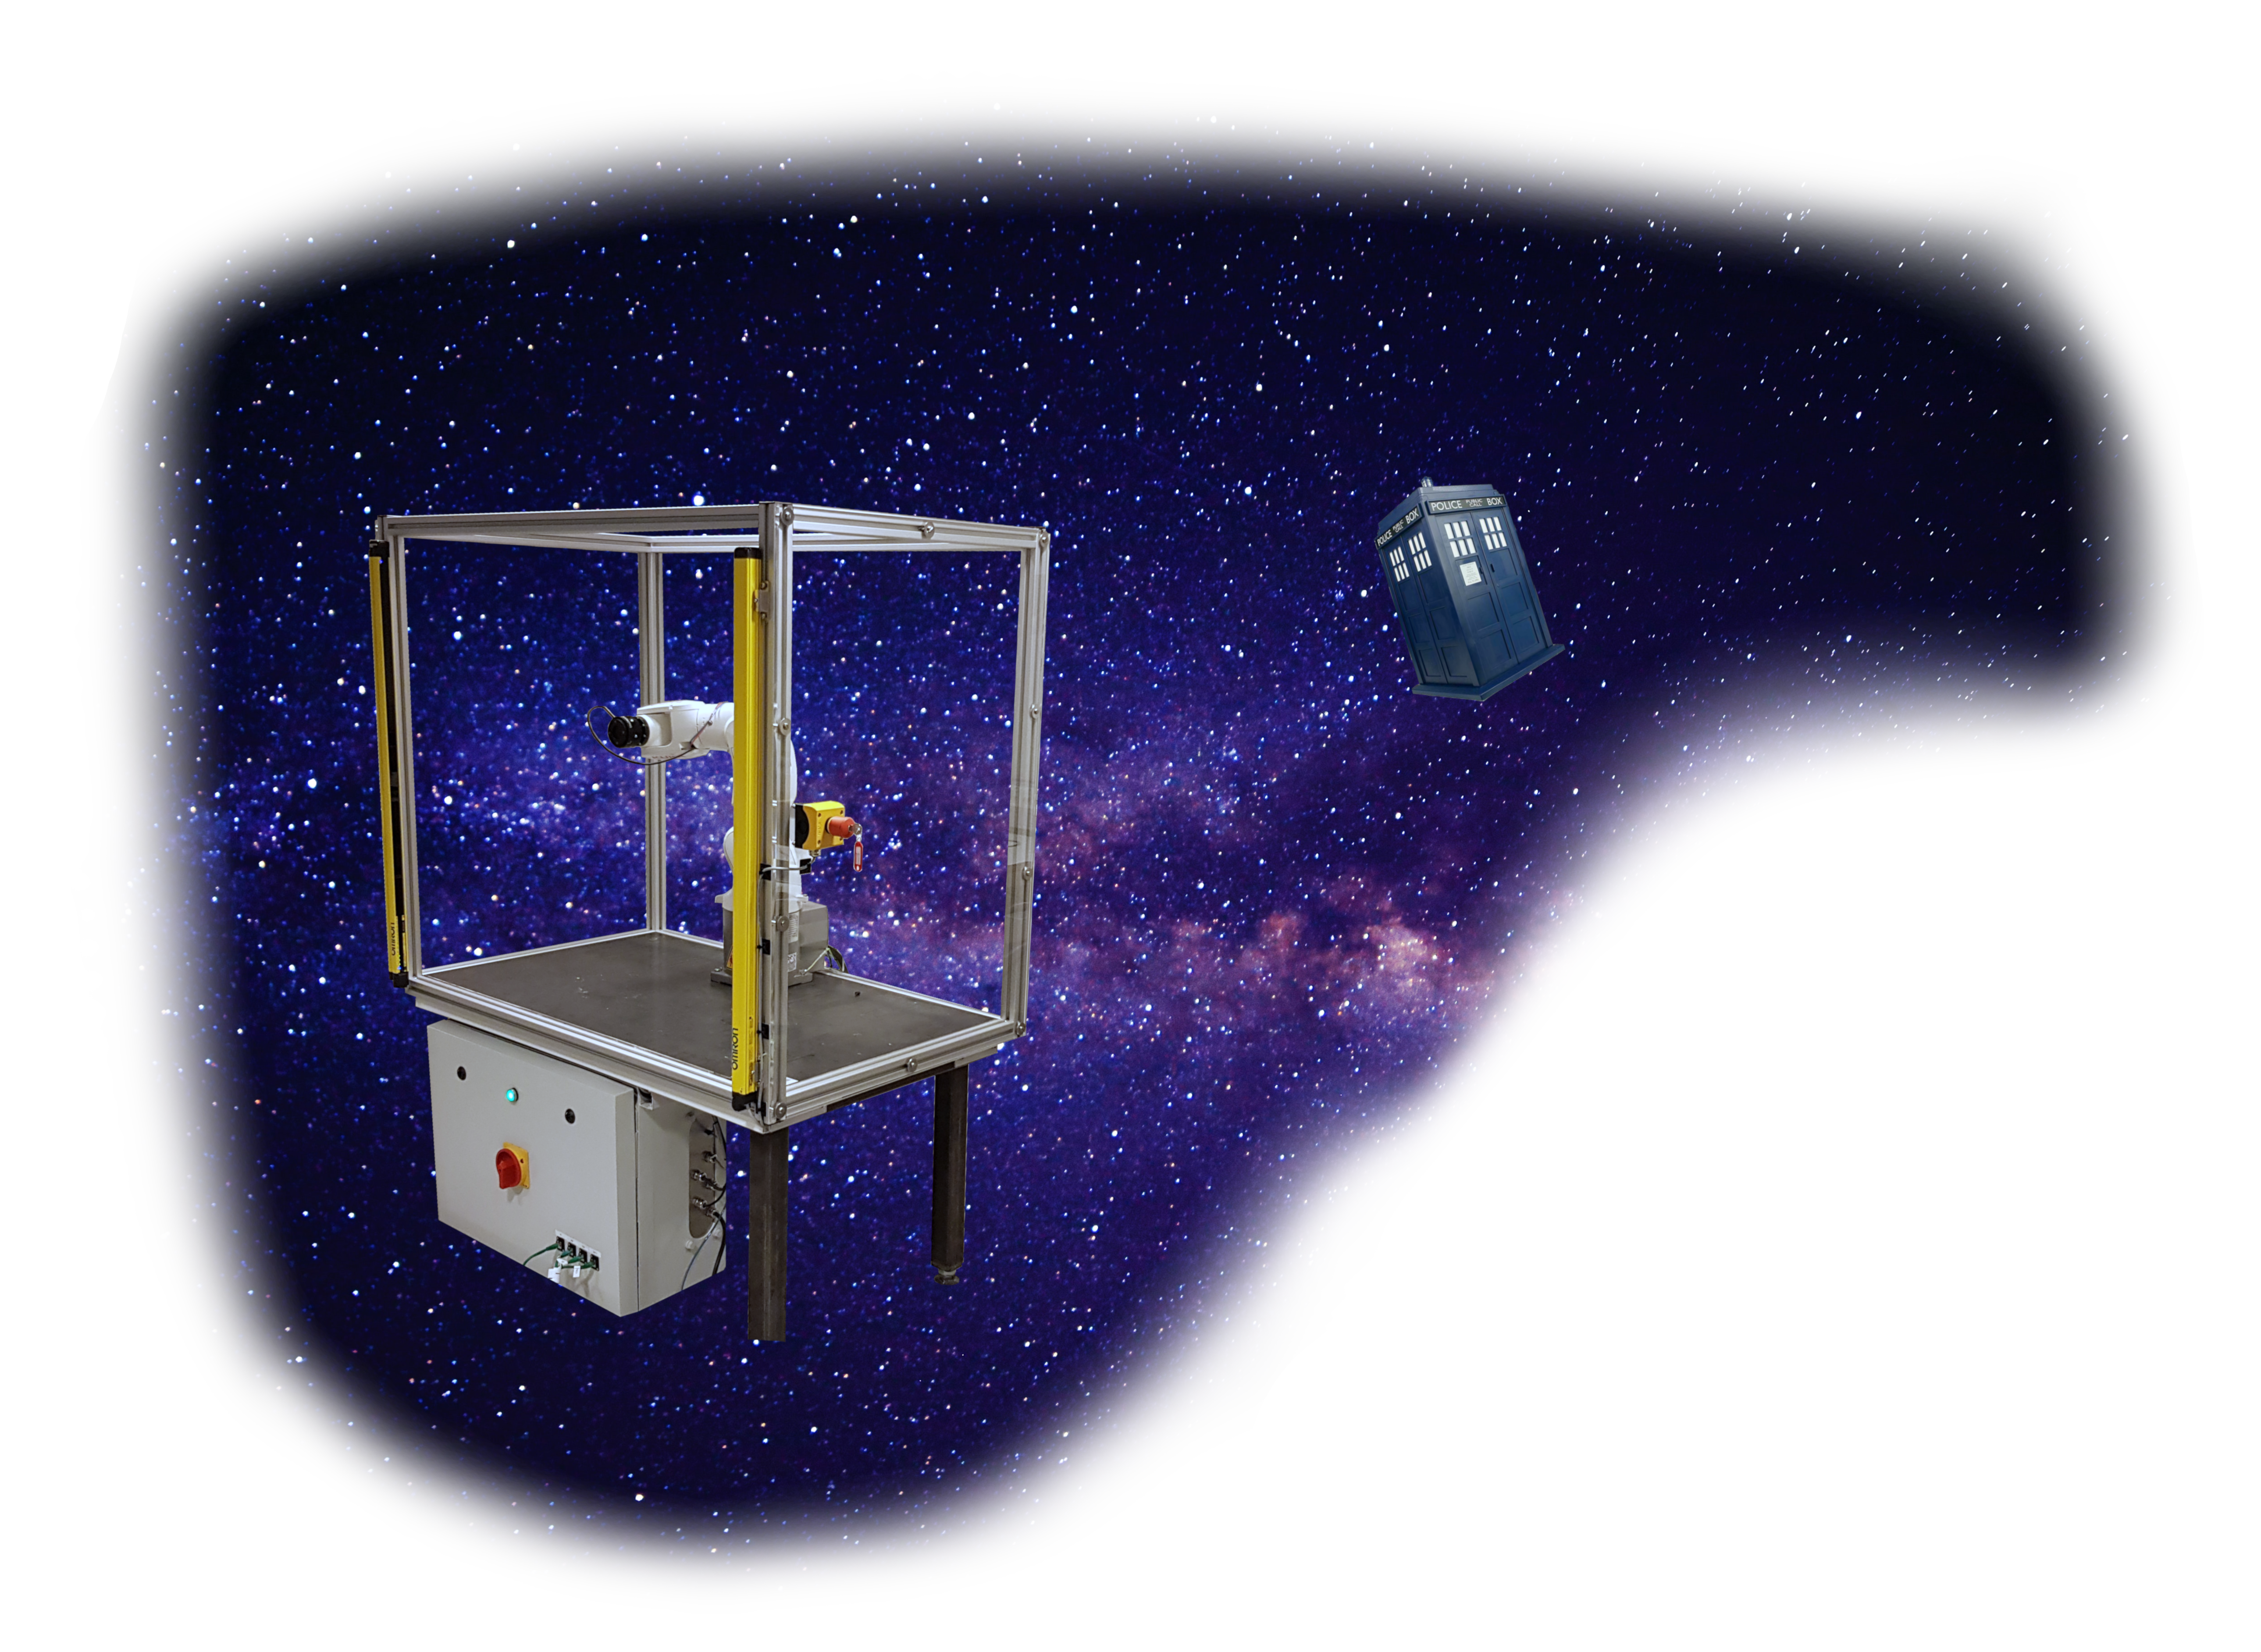
\includegraphics[width=\textwidth]{Pictures/robotlab1_final.png}}
\title{Getting started with Kuka Robot Cell}
\author{Espen Teigen }
\date{March 2019}


\begin{document}

\maketitle

    Github: https://github.com/EspenTeigen/Kuka-KR-C4-commissioning

\newpage
\tableofcontents{}
\newpage


\section{Robot System Diagram}
    \begin{figure}[!h]
        \centering
        \includegraphics[scale=0.3]{"Pictures/Chart".png}
        \caption{System overview. It is not how everything is wired, but conceptual how it connects}
    \end{figure}

\newpage
\section{A brief overview of the Robot-cell and it's parts}
    \subsection{Manipulator}
    
     \begin{figure}[!h]
        \centering
        \includegraphics[scale=0.09]{"Pictures/KR_3_AGILUS".jpg}
        \caption{Kuka KR 3 R540 Agilus}
    \end{figure}
    
    
    Ahh... The manipulator, the part that everyone thinks is the robot, but, no. A robot consists of a controller, end-effector and a manipulator, but I am getting ahead of myself.
    \\\\
    The manipulator is the part that delivers the movement of the tool. In it self, it is just a collection of motors and joints, or as the robotics companies like to say "jointed-arm kinematic system". 
    \\\\
    The manipulator has four pneumatic(input/outputs) near the end-effector. It has an eight-pin M12 contact on the head, where I have used four of the pins on a force torque sensor.  
    
   
    \newpage
    \textcolor{blue}{\textbf{This manipulator is:}
    \begin{itemize}
        \item 6-axis
        \item Capable of moving 3kg of mass(included tool)
        \item Giving a $\pm 0.02mm$ pose repeatabillity
        \item Weighing 26.5kg without a tool
        \item Not very big. It has a maximum reach of 541mm(without tool)
        \item Silent, less then 68dB
        \item Made for pairing with the KR C4 compact controller
        \item What we would call an assembly robot
        \item Really, really fast(See KR 3 R540 Operating Instructions page 12)
        \item In my opinion, really good looking
    \end{itemize}}
    \\\\
    \textcolor{red}{\textbf{It is not:}
    \begin{itemize}
        \item A pot of petunias falling to the ground
        \item \textbf{A toy. When the manipulator is moving at full speed, it has the power to do some major damage to both humans and equipment. Never try to override the safety system, and keep body parts away from the robot cell. Try to avoid standing in front of the robot cell when the robot system are in operation, if you are not sure about how the robot is moving}
         \item A TARDIS\textsuperscript{TM} traveling in wibbly wobbly          timey wimey space. 
    \end{itemize}}
    \\\\
     \textbf{In the back of the manipulator you will find:}
    \begin{itemize}
        \item Air 1-4
        \item X32, this connector is used for mastering(calibrating) the robot
        \item X76, this connector is used for transferring power and data to the connector on the head of the manipulator
        \item One thick cable(X20), used for transferring power to the motors
        \item One thin cable(X21) used for data communication from the controller to the robot. 
        \item One ground wire, used for equipotential bonding with the controller. 
    \end{itemize}
    
  \newpage
  
        \subsubsection{Force-torque sensor}
        \begin{figure}[!h]
            \centering
            \includegraphics[scale=0.2]{"Pictures/FT300".png}
            \caption{Robotiq FT-300}
        \end{figure}
        
        As the section name implies, this is a force-torque sensor. It gives us 3-axis of force, and 3-axis of torque. 
        
          \begin{figure}[!h]
            \centering
            \includegraphics[scale=0.5]{"Pictures/FT300-diagram".png}
            \caption{Axis of sensitivity}
        \end{figure}
        This gives us the possibility to give the robot a feeling of touch. The FT-300 is placed between the manipulator and end-effector.
        \\\\
        This sensor is sending it's data via modbus to a PLC, that transfers the data to the robot system.
       
\newpage
        
        \subsubsection{Pneumatic's}
        The pneumatics on the robot is made of three part. 
        \begin{figure}[!h]
            \centering
            \includegraphics[scale=0.5]{"Pictures/stanley fatmax OL244".jpg}
            \caption{An Stanley Fatmax OL244 air compressor with pressure regulator}
        \end{figure}
        
        \begin{figure}[!h]
            \centering
            \includegraphics[scale=0.3]{"Pictures/festo".jpg}
            \caption{A 5/2 mono-stable solenoid valve}
        \end{figure}
        
        \begin{figure}[!h]
            \centering
            \includegraphics[scale=0.5]{"Pictures/cylinder".jpg}
            \caption{A SMC CD55N12 pneumatic cylinder}
        \end{figure}
        
        \begin{figure}[!h]
            \centering
            \includegraphics[scale=0.5]{"Pictures/air-flow valve".jpg}
            \caption{And two SMC air-flow valves(not to scale, its really small)}
        \end{figure}
        
\newpage

        This setup makes it possible to control the pneumatic valve with digital output 0 from the robot controller. Boolean TRUE extends the cylinder, and boolean FALSE retracts the cylinder. 
        \\\\
        The force of the cylinder is controlled with the pressure regulator on the air compressor. 
        \\\\
        The speed of the cylinder is controlled with the air-flow valves on the back of the manipulator. The one marked +, controls the retraction speed, and the other one controls the extension speed.
        \\\\
          Notice that the air-flow regulators has a check valve that lets air inn to the cylinder. This is because we want to restrict the air-flow out from the cylinder, and not in to it. If you restrict the airflow in, the cylinder will move like you are playing counter strike on a machine with 56k mode, it will lag. 
        
        \begin{figure}
            \centering
            \includegraphics[scale=1]{"Pictures/pneumatic schematic".png}
            \caption{Pneumatic schematic for control of pneumatic cylinder}
        \end{figure}
    
\newpage

        \subsection{Robot Controller}
        
        \begin{figure}[!h]
            \centering
            \includegraphics[scale=0.4]{"Pictures/kr c4 compact".jpg}
            \caption{KR C4 compact}
        \end{figure}
        
        The heart and nerve of the robot system. It is on this one you write you're program, do all the configurations and so on. It reads the rotary encoders on the manipulator, and send control-signals to it. It also handles communication with other robot-controllers, PLC's and computers. It can control servo drives, so on and so forth. If you want to find out more of what it can do, i suggest that you have a look in the documentation; KR C4 compact, Operating Instructions(You can find this on the KRC4 docs standard disk, or on kuka's download center.
        \\\\
        This specific controller has some options that are important to mention. We have the KRC4 compact DC4 FSoE ECAT M/M X55 EN. That mean that this controller is equipped for use with EtherCAT-bus, and supports FSoE(Fail Safe over Ethernet)(made possible with Beckhoff EL6695-1001 Master/master EtherCAT-bridge).  X55 is the power connector to the EtherCAT-bridge inside the controller. I'll describe this under the sub-section EtherCAT further down in the document.
        
\newpage

        \subsubsection{Smart Pad}
        
        \begin{figure}[!h]
            \centering
            \includegraphics[scale=0.5]{"Pictures/smartpad".jpg}
            \caption{Kuka Smart Pad}
        \end{figure}
        
        The first line of interaction with the Kuka robot system. This is a touch pad with OK resolution and horrible touch interface(I suggest you use a Bluetooth keyboard and mouse if you are going to do a lot of work on it).
        \\\\
        But it shines when it comes to moving the robot manipulator. The 6-D mouse on the right side is actually nice to use when you get used to it. The interface is also quit intuitive(in certain areas). I will give a better description how to use it when i start rambling about starting the robot and programming.
        
        \subsubsection{PC-interface}
        \paragraph{Software}
        \subsubsection{EtherCAT}
        
\newpage

    \subsection{Control cabinet}
        \subsubsection{Front panel}
        \subsubsection{PLC}
        \paragraph{PC-interface}
        \paragraph{Software}
        \subsubsection{Pneumatic's}

\newpage

    \subsection{Safety}
        \subsubsection{Do's and dont's }
        \subsubsection{Emergency stop's}
        \subsubsection{Light grid}


\end{document}
